\documentclass[12pt]{article}
\usepackage{graphicx}
\usepackage{amsmath}
\usepackage{gvv-book}
\usepackage{gvv}
\usepackage{enumitem}

\title{\textbf{4.13.13}}
\author{\textbf{EE25BTECH11008 - Anirudh M Abhilash}}
\date{October 11, 2025}

\begin{document}

\maketitle

\section*{Question}

If one of the lines of 
\[
m y^2 + (1 - m^2)xy - m x^2 = 0
\]
is a bisector of the angle between the lines 
\[
xy = 0,
\]
then find the value of $m$.

\section*{Solution}

The given homogeneous equation can be expressed as
\begin{align}
\myvec{x & y}
\myvec{-m & \tfrac{1 - m^2}{2} \\[4pt] \tfrac{1 - m^2}{2} & m}
\myvec{x \\ y} = 0.
\end{align}

Let 
\[
A = \myvec{-m & \tfrac{1 - m^2}{2} \\[4pt] \tfrac{1 - m^2}{2} & m}.
\]

Each line represented by this homogeneous equation passes through the origin, and its direction vector $\vec{v}$ satisfies
\begin{align}
\vec{v}^T A \vec{v} = 0.
\end{align}

For the bisectors of the coordinate axes ($xy=0$), the directions are along $\vec{v_1} = \myvec{1 \\ 1}$ and $\vec{v_2} = \myvec{1 \\ -1}$.

Substituting $\vec{v_1}$,
\begin{align}
\vec{v_1}^T A \vec{v_1} &= \myvec{1 & 1}
\myvec{-m & \tfrac{1 - m^2}{2} \\[4pt] \tfrac{1 - m^2}{2} & m}
\myvec{1 \\ 1} \\[4pt]
&= -m + (1 - m^2) + m = 1 - m^2.
\end{align}

Similarly, substituting $\vec{v_2}$,
\begin{align}
\vec{v_2}^T A \vec{v_2} &= \myvec{1 & -1}
\myvec{-m & \tfrac{1 - m^2}{2} \\[4pt] \tfrac{1 - m^2}{2} & m}
\myvec{1 \\ -1} \\[4pt]
&= -m - (1 - m^2) + m = m^2 - 1.
\end{align}

For either $\vec{v_1}$ or $\vec{v_2}$ to represent a line of the pair,
\begin{align}
1 - m^2 = 0.
\end{align}

Hence,
\begin{align}
m = \pm 1.
\end{align}

\[
\boxed{m = \pm 1}
\]

\begin{figure}[H]\centering
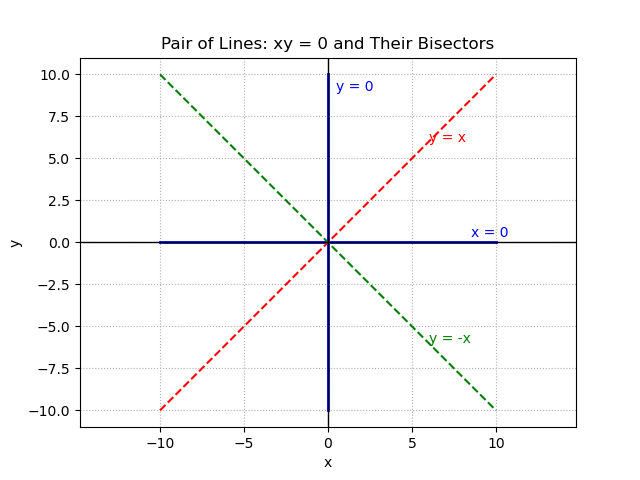
\includegraphics[width=1\columnwidth]{figs/plt.png}
\caption{Lines}
\label{fig:plt}
\end{figure}

\end{document}
